\chapter{Probabilité}
{https://sacado.xyz/qcm/parcours_show_course/0/117120}
{ 

 \begin{CpsCol}
 \textbf{Les savoir-faire} 
 \begin{itemize}
 \item Utiliser le vocabulaire des probabilités : expérience aléatoire, issues, événement, probabilité, événement certain, événement impossible, événement contraire.
 \item Reconnaître des événements contraires et s’en sert pour calculer des probabilités.
 \item Calculer des probabilités.
 \item Savoir que la probabilité d'un événement est un nombre compris entre 0 et 1.
 \item Exprimer des probabilités sous diverses formes.
 
 \end{itemize}
 \end{CpsCol}
}
%
%
%\begin{pageHistoire} 
% 
%En 1585, dans son ouvrage \textbf{La Disme}, Simon Stevin (1548 - 1620) ingénieur et mathématicien flamand, propose une écriture des nombres qui permet de simplifier les calculs (quelquefois très lourds en écriture fractionnaire).\\
%
%Il est considéré comme un précurseur de l'écriture décimale.
% 
%
%\end{pageHistoire} 



%%%%%%%%%%%%%%%%%%%%%%%%%%%%%%%%%%%%%%%%%%%%%%%%%%%%%%%%%%%%%%%%%%%%%%%%%%%%%%%%%%%%
%%%%%%%%%%        Cours             %%%%%%%%%%%%%%%%%%%%%%%%%%%%%%%%%%%%%%%%%%%%%%%%
%%%%%%%%%%%%%%%%%%%%%%%%%%%%%%%%%%%%%%%%%%%%%%%%%%%%%%%%%%%%%%%%%%%%%%%%%%%%%%%%%%%%
\begin{pageCours} 

\section{Vocabulaire}



\begin{DefT}{Expérience aléatoire. Univers. Issue}
Une \textbf{expérience aléatoire}\index{Expérience aléatoire!Probabilité| see{Probabilité}} ou \textbf{épreuve aléatoire!Probabilité| see{Probabilité}}\index{Épreuve aléatoire} est une expérience qui est soumise au hasard. On connait les issues possibles sans savoir laquelle sera réalisée.

Une \textbf{issue} \index{Issue!Probabilité| see{Probabilité}}est le résultat d'une expérience aléatoire.

On appelle \textbf{univers}\index{Univers}, noté $\Omega$ \index{$\Omega$}, l'ensemble de toutes les issues possibles.
\end{DefT}

\begin{ExT}{Lancer de dé}
Je lance un dé équilibré et je note le numéro obtenu sur la face sortie. 
\begin{description}
\item L'\textit{expérience aléatoire} est le Lancer du dé cubique.
\item Une \textit{issue}\index{Issue!Probabilité| see{Probabilité}}  ou \textit{éventualités}\index{Éventualité!Probabilité| see{Probabilité}}  est le numéro obtenu sur la face sortie. Ici, il y a 6 issues possibles.
\item L'\textit{univers} est l'ensemble qui contient les nombres 1; 2; 3; 4; 5; 6. On le note $\Omega = \left\lbrace  1;2;3;4;5;6\right\rbrace $.
\end{description}
\end{ExT}

 
\section{Notion d'évènements}

\begin{DefT}{Évènement}
Un \textbf{évènement} est un ensemble d'issues (ou éventualités)\index{Évènement!Probabilité| see{Probabilité}}.
\end{DefT}


\begin{Rq}
On décrit un évènement par une action.
\end{Rq}


\begin{ExT}{Exemples d'évènements}
Je lance un dé équilibré et je note la face obtenue. 
\begin{description}
\item Obtenir un nombre pair.
\item Obtenir le 6.
\item Obtenir un nombre plus petit que 4.
\end{description}
\end{ExT}

\end{pageCours}


%%%%%%%%%%%%%%%%%%%%%%%%%%%%%%%%%%%%%%%%%%%%%%%%%%%%%%%%%%%%%%%%%%%%%%%%%%%%%%%%%%%%
%%%%%%%%%%   Application directe    %%%%%%%%%%%%%%%%%%%%%%%%%%%%%%%%%%%%%%%%%%%%%%%%
%%%%%%%%%%%%%%%%%%%%%%%%%%%%%%%%%%%%%%%%%%%%%%%%%%%%%%%%%%%%%%%%%%%%%%%%%%%%%%%%%%%%
\begin{pageAD} 

\Sf{Connaître le vocabulaire probabiliste}

\ExoCad{Communiquer.}
 
On lance une pièce de monnaie équilibrée et non truquée.

\begin{enumerate}
\item Quelle est l'expérience aléatoire ? \point{1}
\item Quelles sont les issues ?\point{1}
\item Quel est l'univers ?\point{1}
\end{enumerate}


\ExoCad{Communiquer.}

On considère un jeu de 52 cartes. On en tire une carte au hasard. 
\begin{enumerate}
\item Quelle est l'expérience aléatoire ?\point{1}
\item Donner deux issues possibles.\point{1}
\item Combien l'univers compte-t-il d'issues ?\point{1}
\end{enumerate}


\ExoCad{Communiquer.}

Le bingo est un jeu où il faut deviner 6 nombres tirés au hasard et sans remise parmi 1 et 49 sans se soucier de l'ordre.
\begin{enumerate}
\item Quelle est l'expérience aléatoire ?\point{1}
\item Donner deux issues possibles.\point{1}
\item Donner deux issues impossibles.\point{1}
\end{enumerate}

 
\ExoCad{Représenter. Communiquer.}

On considère l'expérience aléatoire qui consiste à lancer deux dés et faire la somme des faces obtenues.
\begin{enumerate}
\item Décris l'univers.\point{1}
\item Donner deux issues possibles.\point{1}
\end{enumerate}
 


\Sf{Décrire un événement} 

 
\ExoCad{Représenter. Communiquer.}

Dans son armoire, Anis a 3 pantalons : un vert, un bleu et un rouge. Il a aussi 4 chemises : une vert, deux bleues et une rose. Il choisit au hasard un pantalon et une chemise. On s'intéresse aux événements B : "Anis est habillé tout en bleu" et V : "Anis est habillé tout en vert".
\begin{enumerate}
\item Décris l'évènement V ? \point{1}
\item Décris l'évènement B ? \point{1}
\end{enumerate}




\end{pageAD}  




\begin{pageCours}

\begin{DefT}{Évènements particuliers}
\begin{itemize}[leftmargin=*]
\item Un \textbf{évènement élémentaire}\index{Évènement élémentaire!Probabilité| see{Probabilité}} est un ensemble qui contient une seule issue. 
\item Un \textbf{évènement impossible}\index{Évènement impossible!Probabilité| see{Probabilité}} dont on est sûr qu'il ne peut pas se produire.  
\item Un \textbf{évènement certain}\index{Évènement certain!Probabilité| see{Probabilité}}  dont on est sûr qu'il va se produire.  
\end{itemize}

\end{DefT}

\begin{ExT}{Exemples d'évènements}
Je lance un dé équilibré et je note la face obtenue. 

\begin{itemize}[leftmargin=*]
\item L'évènement A : "Obtenir le nombre 5" est un évènement élémentaire.  
\item L'évènement B : "Obtenir le nombre 0" est un évènement impossible.
\item L'évènement C : "Obtenir un nombre compris entre 1 et 6" est un événement certain.
\end{itemize}

\end{ExT}

\section{Probabilité d'un évènement}

\begin{DefT}{Probabilité d'un évènement}
Lorsqu'une expérience est répétée un grand nombre de fois, on assimile la fréquence d'apparition d'un évènement $A$ à sa probabilité\index{Probabilité} et on note la $p(A)$.
\end{DefT}
 
\begin{Pps}
\begin{itemize}[leftmargin=*]
\item La probabilité d'un évènement est la somme des probabilités des évènements élémentaires qui le composent.  
\item La somme des probabilités de tous les évènements élémentaires qui composent l'univers est égale à 1.  
\item La probabilité d'un \textbf{évènement impossible} est égale à 0.  
\item La probabilité d'un \textbf{évènement certain} est égale à 1.  
\end{itemize}
\end{Pps}

\begin{Ex}
Rosi lance un dé truqué dont la probabilité de chaque face est proportionnelle au nombre de la face.
Elle s'intéresse à l'événement F : "Obtenir une face paire".  

  L'évènement $F$ est $\lbrace 2;4;6 \rbrace$, constitué des évènements élémentaires $\lbrace 2 \rbrace$ , $\lbrace 4 \rbrace$ , $\lbrace 6 \rbrace$ 
 

La probabilité de $F$ est donc $p(F) = p\left( \lbrace 2 \rbrace\right) + p\left(\lbrace 4 \rbrace\right) + p\left(\lbrace 6 \rbrace \right)  =\dfrac{2}{21} + \dfrac{4}{21} + \dfrac{6}{21} = \dfrac{12}{21}$


\end{Ex}


\end{pageCours} 
%%%%%%%%%%%%%%%%%%%%%%%%%%%%%%%%%%%%%%%%%%%%%%%%%%%%%%%%%%%%%%%%%%%%%%%%%%%%%%%%%%%%
%%%%%%%%%%   Application directe    %%%%%%%%%%%%%%%%%%%%%%%%%%%%%%%%%%%%%%%%%%%%%%%%
%%%%%%%%%%%%%%%%%%%%%%%%%%%%%%%%%%%%%%%%%%%%%%%%%%%%%%%%%%%%%%%%%%%%%%%%%%%%%%%%%%%%
\begin{pageAD} 

\Sf{Décrire un évènement}

\ExoCad{Chercher.}
 
 
Un jeu de 54 cartes n'est pas truqué. On tire aléatoirement une carte.
\begin{enumerate}
\item Quelles issues composent l'évènement R : "Obtenir un roi" ?\point{2}
\item Déterminer un évènement élémentaire. \point{1}
\item Déterminer un évènement impossible.\point{1}
\end{enumerate}



\Sf{Calculer une probabilité}

\ExoCad{Chercher.}
 
 
Un jeu de 32 cartes n'est pas truqué. On titre aléatoirement une carte.
\begin{enumerate}
\item Déterminer la probabilité de tirer un trèfle.
\item Déterminer la probabilité de tirer un roi.
\item Déterminer la probabilité de tirer le roi de cœur.
\end{enumerate}
 

 
 

\ExoCad{Chercher. Communiquer.}

L'expérience consiste à choisir un élève au hasard. 

\begin{enumerate}
\item Complète le tableau ci-desous :

\begin{tabular}{|c|c|c|c|}
\hline 
 & Sportif & Non sportif &  \\ 
\hline 
Filles & $35$ &   & $55$ \\ 
\hline 
Garçons & $25$ & $20$ &  \\ 
\hline 
 &  &  & $100$ \\ 
\hline 
\end{tabular} 


\item Quelle est la probabilité que ce soit un sportif ? \point{1}
\item Quelle est la probabilité que ce soit une fille sportive ?\point{1}

\end{enumerate}

\ExoCad{Calculer.}
 
Lors de multiples lancers de dés, on note les fréquences d'apparition de chaque face. 

\begin{tabular}{|c|c|c|c|c|c|c|}
\hline 
Face & $1$ & $2$ & $3$ & $4$  & $5$ & $6$ \\ 
\hline 
Fréquence & $0.12$ & $0.2$ & $\ldots\ldots$ & $0.18$  & $0.17$ & $0.15$ \\ 
\hline 
\end{tabular}

\begin{enumerate}
\item Complète le tableau ci-dessus.
\item Quelle est la probabilité de l'événement P :"Obtenir un nombre inférieur à 4" ?\point{1}

\end{enumerate}

 

\end{pageAD} %%%%%%%%%%%%%%%%%%%%%%%%%%%%%%%%%%%%%%%%%%%%%%%%%%%%%%%%%%%%%%%%%%%%%%%%%%%%%%%%%%%%
%%%%%%%%%%   Application directe    %%%%%%%%%%%%%%%%%%%%%%%%%%%%%%%%%%%%%%%%%%%%%%%%
%%%%%%%%%%%%%%%%%%%%%%%%%%%%%%%%%%%%%%%%%%%%%%%%%%%%%%%%%%%%%%%%%%%%%%%%%%%%%%%%%%%%
%
%\begin{pageCours}
%
%\section{Représentation d'une expérience}
%
%\begin{DefT}{Arbre de dénombrement}
%
%Pour représenter un expérience aléatoire, on peut utiliser un arbre de dénombrement\index{Arbre de dénombrement}. Cette représentation décrit toutes les issues possibles de l'expérience.
%
%\end{DefT}
% 
%
%
%
%\begin{ExT}{Arbre de dénombrement}
%
%Dans une urne, il y a 2 boules vertes et 5 boules rouges.
% \begin{description}
%\item Si une boule verte est tirée alors le joueur tire une autre boule.
%\item Si une boule rouge est tirée alors le joueur perd la partie.
%\end{description}
%
%Représentons cette expérience par un arbre de dénombrement.
%
%
%
%
%
%
%
%
%
%\end{ExT}
% 
%
%
%
%\end{pageCours} 
%%%%%%%%%%%%%%%%%%%%%%%%%%%%%%%%%%%%%%%%%%%%%%%%%%%%%%%%%%%%%%%%%%%%%%%%%%%%%%%%%%%%%
%%%%%%%%%%%   Application directe    %%%%%%%%%%%%%%%%%%%%%%%%%%%%%%%%%%%%%%%%%%%%%%%%
%%%%%%%%%%%%%%%%%%%%%%%%%%%%%%%%%%%%%%%%%%%%%%%%%%%%%%%%%%%%%%%%%%%%%%%%%%%%%%%%%%%%%
%\begin{pageAD} 
%
%\Sf{Reconnaître une situation de  }
%
%
%
%\end{pageAD} 
%%%%%%%%%%%%%%%%%%%%%%%%%%%%%%%%%%%%%%%%%%%%%%%%%%%%%%%%%%%%%%%%%%%%%%%%%%%%%%%%%%%%
%%%%%%%%%%        Parcours 1    %%%%%%%%%%%%%%%%%%%%%%%%%%%%%%%%%%%%%%%%%%%%%%%%%%%%
%%%%%%%%%%%%%%%%%%%%%%%%%%%%%%%%%%%%%%%%%%%%%%%%%%%%%%%%%%%%%%%%%%%%%%%%%%%%%%%%%%%%
\begin{pageParcoursu} 





\ExoCu{Raisonner.}
 

On jette une pièce de monnaie en l'air et on regarde la pièce posée sur le sol. On s'intéresse à l'événement $F$: "La pièce montre la face Face". Quelle est la probabilité de l'événement $F$ ?\point{2}

 


 \ExoCu{Calculer.}


Une urne contient 1 boule rouge et 4 boules oranges indiscernables au toucher. 

Calculer la probabilité de tirer une boule orange. \point{3}

 





\ExoCu{Raisonner. Calculer.}
 
\begin{minipage}{.68\linewidth}
Une roue est composée de 8 secteurs angulaires superposables de couleurs différentes. Une aiguille tourne au hasard et s'arrête sur un des secteurs. On note la couleur obtenue.

\begin{enumerate}
\item Quelle est la probabilité que la couleur soit jaune ? \point{1}
\item Quelle est la probabilité que la couleur soit rose ?\point{1}
\end{enumerate}
\end{minipage}
\hfill
\begin{minipage}{.28\linewidth}


\definecolor{ffffff}{rgb}{1.,1.,1.}
\definecolor{ffqqff}{rgb}{1.,0.,1.}
\definecolor{ffdxqq}{rgb}{1.,0.8431372549019608,0.}
\definecolor{qqqqff}{rgb}{0.,0.,1.}
\begin{tikzpicture}[line cap=round,line join=round,>=triangle 45,x=1.0cm,y=1.0cm]
\clip(-2.08,-1.14) rectangle (2.04,3.3);
\draw [shift={(0.,1.)},line width=2.pt,color=qqqqff,fill=qqqqff,fill opacity=0.7]  (0,0) --  plot[domain=0.:0.7853981633974483,variable=\t]({1.*2.*cos(\t r)+0.*2.*sin(\t r)},{0.*2.*cos(\t r)+1.*2.*sin(\t r)}) -- cycle ;
\draw [shift={(0.,1.)},line width=2.pt,color=ffdxqq,fill=ffdxqq,fill opacity=0.7]  (0,0) --  plot[domain=0.7853981633974483:1.5707963267948966,variable=\t]({1.*2.*cos(\t r)+0.*2.*sin(\t r)},{0.*2.*cos(\t r)+1.*2.*sin(\t r)}) -- cycle ;
\draw [shift={(0.,1.)},line width=2.pt,color=ffqqff,fill=ffqqff,fill opacity=0.7]  (0,0) --  plot[domain=1.5707963267948966:2.356194490192345,variable=\t]({1.*2.*cos(\t r)+0.*2.*sin(\t r)},{0.*2.*cos(\t r)+1.*2.*sin(\t r)}) -- cycle ;
\draw [shift={(0.,1.)},line width=2.pt,color=ffdxqq,fill=ffdxqq,fill opacity=0.7]  (0,0) --  plot[domain=2.356194490192345:3.141592653589793,variable=\t]({1.*2.*cos(\t r)+0.*2.*sin(\t r)},{0.*2.*cos(\t r)+1.*2.*sin(\t r)}) -- cycle ;
\draw [shift={(0.,1.)},line width=2.pt,color=ffqqff,fill=ffqqff,fill opacity=0.7]  (0,0) --  plot[domain=3.141592653589793:3.9269908169872414,variable=\t]({1.*2.*cos(\t r)+0.*2.*sin(\t r)},{0.*2.*cos(\t r)+1.*2.*sin(\t r)}) -- cycle ;
\draw [shift={(0.,1.)},line width=2.pt,color=ffdxqq,fill=ffdxqq,fill opacity=0.7]  (0,0) --  plot[domain=3.9269908169872414:4.71238898038469,variable=\t]({1.*2.*cos(\t r)+0.*2.*sin(\t r)},{0.*2.*cos(\t r)+1.*2.*sin(\t r)}) -- cycle ;
\draw [shift={(0.,1.)},line width=2.pt,color=ffqqff,fill=ffqqff,fill opacity=0.7]  (0,0) --  plot[domain=4.71238898038469:5.497787143782138,variable=\t]({1.*2.*cos(\t r)+0.*2.*sin(\t r)},{0.*2.*cos(\t r)+1.*2.*sin(\t r)}) -- cycle ;
\draw [shift={(0.,1.)},line width=2.pt,color=ffdxqq,fill=ffdxqq,fill opacity=0.7]  (0,0) --  plot[domain=-0.7853981633974483:0.,variable=\t]({1.*2.*cos(\t r)+0.*2.*sin(\t r)},{0.*2.*cos(\t r)+1.*2.*sin(\t r)}) -- cycle ;
\draw [->,line width=5.2pt,color=ffffff] (0.,1.) -- (1.54,1.7);
\end{tikzpicture}

\end{minipage}


 \ExoCu{Raisonner.}
 
 On lance un dé équilibré à 20 faces numérotées de 1 à 20. La probabilité pour que le numéro tiré soit inférieur ou égal à 5 est 
 
 $$ \dfrac{1}{20} \quad\quad \dfrac{5}{20} \quad\quad \dfrac{1}{5} \quad\quad \dfrac{5}{6} $$
 
 \textit{Entoure la bonne réponse}
 

 \ExoCu{Raisonner.}
 

Une collectionneuse compte ses cartes Pokémon afin de les revendre. Elle possède 252 cartes de type « feu » et 156 cartes de type « terre ». Elle choisit une carte au hasard parmi toutes ses cartes. On suppose les cartes indiscernables au toucher.
Calculer la probabilité que ce soit une carte de type « terre ». \point{2}

\ExoCu{Calculer.}

Dans une urne, il y a $6$ boules vertes, $2$ rouges et $1$ noire indiscernables au toucher. On tire une boule au hasard. 


\begin{enumerate}
\item Calcule la probabilité de l'événement V:"Tirer une boule verte". \point{1}
\item Calcule la probabilité de l'événement R:"Tirer une boule rouge". \point{1}
\end{enumerate}

\end{pageParcoursu}
%%%%%%%%%%%%%%%%%%%%%%%%%%%%%%%%%%%%%%%%%%%%%%%%%%%%%%%%%%%%%%%%%%%%%%%%%%%%%%%%%%%%
%%%%%%%%%%        Parcours 2    %%%%%%%%%%%%%%%%%%%%%%%%%%%%%%%%%%%%%%%%%%%%%%%%%%%%
%%%%%%%%%%%%%%%%%%%%%%%%%%%%%%%%%%%%%%%%%%%%%%%%%%%%%%%%%%%%%%%%%%%%%%%%%%%%%%%%%%%%
\begin{pageParcoursd} 


\ExoCd{Chercher. Raisonner.}
 
 
Dans la classe il y a $25$ élèves dont $19$ sont droitiers, aucun n'est ambidextre. On choisit au hasard un élève.
\begin{enumerate}[leftmargin=*]
\item Décris l'expérience.\point{2}
\item Détermine la probabilité qu'il soit gaucher.\point{1}
\item Détermine la probabilité qu'il soit droitier.\point{1}
\end{enumerate}
 
 
 
\ExoCd{Raisonner. Communiquer.}
 
 \begin{minipage}{.7\linewidth}
 
 On considère une urne contenant des boules blanches ou grises, et numérotées ci-contre :
  \begin{itemize}[leftmargin=*]
\item Si on s'intéresse à la couleur de la boule, quelles sont les issues possibles ?\point{1}
\item Si on s'intéresse au numéro écrit sur la boule, quelles sont les issues possibles ?\point{1}
\item Donne un événement certain de se réaliser. \point{1}
\item Donne un événement impossible. \point{1}
 \end{itemize}

 \end{minipage}
 \begin{minipage}{.3\linewidth}
\includegraphics[scale=1]{FIG/boule.jpg} 

 \end{minipage}
 
\ExoCd{Calculer. Communiquer.}

La probabilité de gagner à un jeu est égale $0,4$. Calcule la probabilité de perdre. \point{3}

 
\ExoCd{Représenter. Calculer.}

Une urne contient $9$ boules indiscernables au toucher : $3$ boules noires, $4$ boules blanches, $2$ boules rouges.

Quelle est la probabilité de ne pas tirer de boule noire ? \point{2}

\ExoCd{Représenter. Raisonner.}

Deux urnes opaques contiennent des boules de couleur, indiscernables au toucher.
Voici la composition de chaque urne :
\begin{itemize}
\item Urne A : 20 boules dont 8 boules bleues
\item Urne B : 11 boules bleues et 14 boules vertes
\end{itemize}
Que dire de l'affirmation : "on a plus de chance de tirer au hasard une boule bleue dans l'urne B que dans l'urne A." ? \point{2}







\end{pageParcoursd}
%%%%%%%%%%%%%%%%%%%%%%%%%%%%%%%%%%%%%%%%%%%%%%%%%%%%%%%%%%%%%%%%%%%%%%%%%%%%%%%%%%%%
%%%%%%%%%%        Parcours 3    %%%%%%%%%%%%%%%%%%%%%%%%%%%%%%%%%%%%%%%%%%%%%%%%%%%%
%%%%%%%%%%%%%%%%%%%%%%%%%%%%%%%%%%%%%%%%%%%%%%%%%%%%%%%%%%%%%%%%%%%%%%%%%%%%%%%%%%%%
\begin{pageParcourst}

\ExoCt{Calculer.}

On lance un dé truqué dont la probabilité de chaque face est donnée dans le tableau.

\begin{enumerate}[leftmargin=*]

\item Compléter le tableau

\begin{tabular}{|c|c|c|c|c|c|c|c|}
\hline 
Face & 1 & 2 & 3 & 4 & 5 & 6 & somme \\ 
\hline 
Probabilité & $\dfrac{1}{21}$ & $\dfrac{2}{21}$  & $\dfrac{3}{21}$  &  $\ldots$   & $\dfrac{5}{21}$  & $\dfrac{6}{21}$  & $1$ \\ 
\hline 
\end{tabular}

\item Est-il plus probable d'obtenir une face paire ou une des faces 5 ou 6 ? \point{5}

\end{enumerate}

\ExoCt{Représenter. Calculer.}
 
Dans un centre de vacances, il y a 400 personnes. 
 
\begin{enumerate}[leftmargin=*]

\item Complète le tableau

\begin{tabular}{|c|c|c|c|c|c|c|}
\hline 
  & Bungalow  & Tente & Mobile home & Total \\ 
\hline 
Femmes   & $280$ & $45$ &  $\ldots\ldots$ & $\ldots\ldots$ \\ 
\hline 
Hommes  & $250$ & $\ldots\ldots$ &  $110$ & $\ldots\ldots$ \\ 
\hline 
Total  &  $\ldots\ldots$ & $120$ &  $\ldots\ldots$ & $900$ \\ 
\hline 
\end{tabular}

On choisit un touriste au hasard de ce centre de vacances.
 
\item Quelle est la probabilité de choisir une femme  ?\point{1}
\item Quelle est la probabilité de choisir un homme qui dort dans une tente ?\point{1}
\end{enumerate}




\ExoCt{Représenter. Calculer.}

\begin{minipage}{.5\linewidth}
Dans une urne, il y a $6$ boules vertes, $2$ rouges et $1$ noire indiscernables au toucher. On tire $2$ boules successivement et sans remise.
\end{minipage}
\begin{minipage}{.5\linewidth}
\vspace{3cm}
\end{minipage}
\begin{enumerate}[leftmargin=*]
\item Calcule la probabilité de l'événement A : "Tirer $2$ boules vertes". \point{1}
\item Calcule la probabilité de l'événement B : "Tirer une boule rouge puis une boule verte". \point{1}
\item Calcule la probabilité de l'événement C : "Tirer une boule rouge et une boule verte". \point{1}
\item Calcule la probabilité de l'événement D : "Tirer $2$ boules noires". \point{1}
\end{enumerate}



\end{pageParcourst}
%%%%%%%%%%%%%%%%%%%%%%%%%%%%%%%%%%%%%%%%%%%%%%%%%%%%%%%%%%%%%%%%%%%%%%%%%%%%%%%%%%%%
%%%%%%%%%%        Parcours 3    %%%%%%%%%%%%%%%%%%%%%%%%%%%%%%%%%%%%%%%%%%%%%%%%%%%%
%%%%%%%%%%%%%%%%%%%%%%%%%%%%%%%%%%%%%%%%%%%%%%%%%%%%%%%%%%%%%%%%%%%%%%%%%%%%%%%%%%%%
\begin{pageInfo}


\ExoCu{Calculer. Communiquer.}


\begin{minipage}{.5\linewidth}
 Ana et ses amies effectuent chacune $200$ lancers d'une pièce de monnaie. 
 
 \begin{tabular}{|c|c|c|c|c|}
 \hline 
 & Ana & Jeanne & Sarah & Imen \\ 
 \hline 
 Pile & $120$ & $103$ & $91$ & $82$ \\ 
 \hline 
 Face & $80$ & $97$ & $109$ & $118$ \\ 
 \hline
 \end{tabular} 
 
\end{minipage}
\begin{minipage}{.5\linewidth}

1.  Construis sur une feuille tableur ce table. 

 
\begin{tabular}{|c|c|c|c|c|c|}
\hline 
   & $1$ & $2$ & $3$ & $4$ & $5$\\
\hline 
\textbf{A} & Nombre de lancers & $20$ & $40$ & $60$ & $80$ \\ 
 \hline 
 \textbf{B} & Nombre de Pile & $12$ &  &  &    \\ 
 \hline 
 \textbf{C} &  Nombre de Face & $8$ & &  &      \\ 
 \hline 
 \end{tabular} 

 
Quelle formule doit-on écrire dans la cellule \textbf{B3} pour copier coller les résultats ? \point{1}

\end{minipage}

2. Complète le diagramme cartésien suivant.
 
 
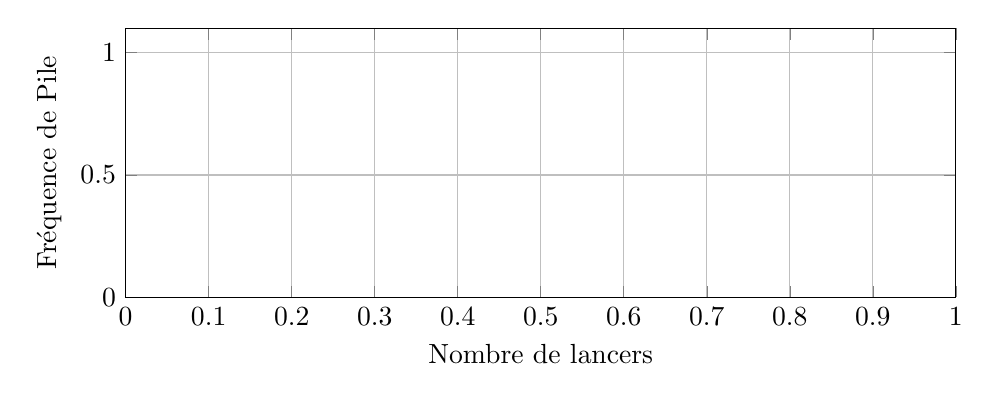
\begin{tikzpicture}
  \begin{axis}[
  	grid=major,
    xlabel={Nombre de lancers},
    ylabel={Fréquence de Pile},
	ytick={0.5,1},
	ymin=0,
	xmin=0,
	xmax=800,
	xtick={200,400,600,800},
    width=\linewidth,
    height=5cm,
  ]
  \end{axis}
\end{tikzpicture}
 
3. Que dire de la pièce de Ana  ? \point{1}


\ExoCd{Calculer.}
 
 On lance un dé et on s'intéresse à la probabilité d'obtenir la face 1.
\begin{enumerate}[leftmargin=*]	
\item Estime cette probabilité.
\item Ouvrir une feuille de calcul dans un tableur.
\begin{enumerate}
\item Avec 100 valeurs
\begin{enumerate}
\item Écrire dans la cellule A1 :"=ALEA.ENTRE.BORNES(1;6)". 

Que fait l'instruction ALEA.ENTRE.BORNES ?
\item Glisser copier la cellule A1 dans la plage "A1:A10" puis la plage "A1:A10" dans "A1:J10".
\item Écrire dans la cellule K1 :"=NB.SI(A1:I10;1)". Que fait l'instruction NB.SI ?
\item Calculer dans la cellule L1 la fréquence d'apparition du nombre 1 dans "A1:J10".
\item Que constates-tu par rapport à ton estimation ?
\end{enumerate}
\item Avec 1000 valeurs
\begin{enumerate}
\item Glisser copier la ligne "A1:I1" jusqu'à la ligne "A100:I100".
\item Modifier la cellule K1 pour obtenir le nombre d'apparaitre de 1 parmi ces \np{1000} valeurs.
\item Modifier la cellule L1 pour calculer la fréquence d'apparition du nombre 1 dans la plage A1:J100.
\item Que constates-tu par rapport à ton estimation ?
\end{enumerate}
\item Avec 10000 valeurs
\begin{enumerate}
\item Glisser copier la ligne "A1:I1" jusqu'à la ligne "A1000:I1000".
\item Modifier la cellule K1 pour obtenir le nombre d'apparition de 1 parmi ces \np{10000} valeurs.
\item Modifier la cellule L1 pour calculer la fréquence d'apparition du nombre 1 dans la plage A1:J1000.
\item Que constates-tu par rapport à ton estimation ?
\end{enumerate}
\end{enumerate}
\end{enumerate}


\end{pageInfo}
%%%%%%%%%%%%%%%%%%%%%%%%%%%%%%%%%%%%%%%%%%%%%%%%%%%%%%%%%%%%%%%%%%%%%%%%%%%%%%%%%%%%
%%%%%%%%%%   Auto-evaluation    %%%%%%%%%%%%%%%%%%%%%%%%%%%%%%%%%%%%%%%%%%%%%%%%%%%%
%%%%%%%%%%%%%%%%%%%%%%%%%%%%%%%%%%%%%%%%%%%%%%%%%%%%%%%%%%%%%%%%%%%%%%%%%%%%%%%%%%%%
\begin{pageAuto}
 
\ExoAuto
 

 \begin{enumerate}
\item A-t-on plus de chance de tirer une boule blanche dans :
\begin{description}
\item \textbf{a.} une urne A qui contient 3 boules toutes blanches ?
\item ou
\item \textbf{b.} une urne B qui contient 500 boules blanches et une boule rouge ?
\end{description}
\item A-t-on plus de chance de tirer une boule blanche ou une boule noire dans chacune  
des urnes ci-dessous ?
\end{enumerate}


\begin{tikzpicture}[line cap=round,line join=round,>=triangle 45,x=0.7730771794105831cm,y=0.7730771794105831cm]
\clip(-4.705366855860613,-10.542921242507836) rectangle (14.697611785206563,-1.212189475625239);
\draw [fill=black,fill opacity=1.0] (11.669758430390349,-7.515067887691629) circle (1cm);
\draw [fill=black,fill opacity=1.0] (1.6284080190100414,-7.051620945627923) circle (1cm);
\draw [->,line width=5.2pt] (-3.,3.) -- (9.,3.);
\draw [rotate around={5.24181994697955:(-1.93,3.84)},color=ffqqqq,fill=ffqqqq,fill opacity=0.59] (-1.93,3.84) ellipse (1.0259941224374605cm and 0.5801909002249424cm);
\draw (-2.9133720132142815,4.071105663900999) node[anchor=north west] {improbable};
\draw [rotate around={5.241819946979561:(0.09,2.1)},color=ffdxqq,fill=ffdxqq,fill opacity=0.59] (0.09,2.1) ellipse (1.0259941224374631cm and 0.5801909002249442cm);
\draw (-1.2140665589806914,2.3409037468631673) node[anchor=north west] {peu probable};
\draw [rotate around={5.241819946979548:(4.85,3.76)},color=qqqqff,fill=qqqqff,fill opacity=0.22] (4.85,3.76) ellipse (1.0259941224374611cm and 0.5801909002249431cm);
\draw (3.9456427293285734,4.0402092010967525) node[anchor=north west] {probable};
\draw [rotate around={5.241819946979548:(6.89,2.34)},color=black,fill=black,fill opacity=0.23] (6.89,2.34) ellipse (1.0259941224374616cm and 0.5801909002249431cm);
\draw (5.614051720757916,2.61897191210139) node[anchor=north west] {très probable};
\draw [color=black](8.332940447531662,4.225587977922235) node[anchor=north west] {Certain};
\draw [->,line width=1.2pt] (8.98,3.74) -- (8.98,2.98);
\draw (-4.,-2.)-- (-4.,-10.);
\draw (-4.,-10.)-- (4.,-10.);
\draw (4.,-10.)-- (4.,-2.);
\draw (6.,-2.)-- (6.,-10.);
\draw (6.,-10.)-- (14.,-10.);
\draw (14.,-10.)-- (14.,-2.);
\draw(-2.07916751749961,-7.391482036474641) circle (0.5cm);
\draw(7.776804117055214,-4.363628681658434) circle (0.5cm);
\draw(7.529632414621236,-7.360585573670393) circle (0.5cm);
\draw(11.360793802347878,-3.7765958883777406) circle (0.5cm);
\begin{scriptsize}
\draw [color=black] (-3.,3.)-- ++(-4.5pt,0 pt) -- ++(9.0pt,0 pt) ++(-4.5pt,-4.5pt) -- ++(0 pt,9.0pt);
\draw [color=black] (3.,3.)-- ++(-4.5pt,0 pt) -- ++(9.0pt,0 pt) ++(-4.5pt,-4.5pt) -- ++(0 pt,9.0pt);
\end{scriptsize}
\end{tikzpicture}

\ExoAuto
 

Une urne contient 90 boules indiscernables au toucher, dont 20 sont bleues, 30 rouges et le reste des boules sont vertes. On tire une seule boule de cette urne.

\begin{enumerate}
\item Quelle est la probabilité de tirer une boule verte ?\point{1}
\item Quelle est la probabilité de tirer une boule bleue ?\point{1}
\item Quelle est la probabilité de tirer une boule blanche ?\point{1}
\end{enumerate}



\end{pageAuto}
%%%%%%%%%%%%%%%%%%%%%%%%%%%%%%%%%%%%%%%%%%%%%%%%%%%%%%%%%%%%%%%%%%%%%%%%%%%%%%%%%%%%
% Parcours 3
%%%%%%%%%%%%%%%%%%%%%%%%%%%%%%%%%%%%%%%%%%%%%%%%%%%%%%%%%%%%%%%%%%%%%%%%%%%%%%%%%%%%
\begin{pageBrouillon} 
 
\ligne{30}

\end{pageBrouillon}


